\chapter*{Úvod}
\addcontentsline{toc}{chapter}{Úvod}

\section{Magnetooptické jevy a jejich využití}
Jako první se jevy, kdy látka ovlivňovala šíření světla v závislosti na magnetickém poli, zabýval Faraday. Roku 1845 objevil, že lineárně polarizované světlo stáčí svou rovinu polarizace při průchodu skleněným válcem v magnetickém poli. To mimo jiné vedlo k potvrzení spojitosti světla a magnetismu. K podobnému závěru došel i Kerr, který však narozdíl od Faradaye nezkoumal průchod, ale odtaz světla.

Magnetooptické jevy se dají pozorovat, jak bylo uvedeno výše, buď při průchodu, bebo odrazu, přičemž naším cílem je zkoumání druhého, častěji zavého Kerrova jevu. Co se týče geometrie, máme na výběr ze tří základních konfigurací. Jedná se o polární, longitudiální a transversální. Jejich schěma naleznete na obrázku (\ref{schema geo}). Jakákoliv jiná poloha vektoru magetizace se dá složit z těchto tří příadů. V rámci této práce se budeme zabývat poze polárním Kerrovýj efektem.

\begin{figure}
    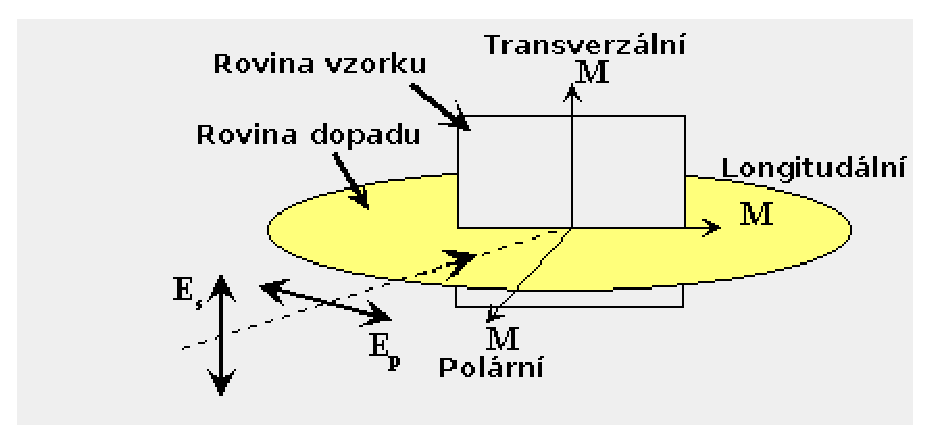
\includegraphics{img/polar.eps}
    \caption{Schéma geometrie Kerrova magnetooptického jevu.}
    \label{schema geo}
\end{figure}

\section{Aplikace magnetoopticky}
Magnetooptika má jakožto velmi široký obor i široké množství uplatnění. Mezi nejznámější patří magnetooptická sektroskopie, umožňující zkoumání struktur o rozměrech řádově nanometrů. Mezi další aplikace patří 3D displaye využívající magnetické nanovrstvy. Pixely těchto displayů se pohybují pod 1 $\mu$m. Jako poslední uvádím magnetooptické izolátory, které propouští světlo pouze jedním směrem. Tyto zařízení jsou nejčastěji používány u výkonných laserů, kde zabraňují návratu svazku zpět do laseru.
